% use the answers clause to get answers to print; otherwise leave it out.
\documentclass[11pt,addpoints,answers]{exam}
%\documentclass[11pt,addpoints]{exam}
\RequirePackage{amssymb, amsfonts, amsmath, latexsym, verbatim, xspace, 
setspace, wasysym}
\usepackage{graphicx}

% By default LaTeX uses large margins.  This doesn't work well on exams; problems
% end up in the "middle" of the page, reducing the amount of space for students
% to work on them.
\usepackage[margin=1in]{geometry}
\usepackage{enumerate}
\usepackage[hidelinks]{hyperref}
\usepackage{subfig}

% Here's where you edit the Class, Exam, Date, etc.
\newcommand{\class}{NPRE 560}
\newcommand{\term}{Fall 2024}
\newcommand{\assignment}{HW 3}
\newcommand{\duedate}{2024.10.23}
%\newcommand{\timelimit}{50 Minutes}
\newcommand{\StudentName}{Oleksandr Yardas} %Please include your name here

\newcommand{\nth}{n\ensuremath{^{\text{th}}} }
\newcommand{\ve}[1]{\ensuremath{\mathbf{#1}}}
\newcommand{\Macro}{\ensuremath{\Sigma}}
\newcommand{\vOmega}{\ensuremath{\hat{\Omega}}}

% For an exam, single spacing is most appropriate
\singlespacing
% \onehalfspacing
% \doublespacing

% For an exam, we generally want to turn off paragraph indentation
\parindent 0ex

%\unframedsolutions

\begin{document} 

% These commands set up the running header on the top of the exam pages
\pagestyle{head}
\firstpageheader{}{}{}
\runningheader{\class}{\assignment\ - Page \thepage\ of \numpages}{Due \duedate}
\runningheadrule

\class \hfill \StudentName \hfill \term \\
\assignment \hfill Due \duedate\\
\rule[1ex]{\textwidth}{.1pt}
%\hrulefill

%%%%%%%%%%%%%%%%%%%%%%%%%%%%%%%%%%%%%%%%%%%%%%%%%%%%%%%%%%%%%%%%%%%%%%%%%%%%%%%%%%%%%
%%%%%%%%%%%%%%%%%%%%%%%%%%%%%%%%%%%%%%%%%%%%%%%%%%%%%%%%%%%%%%%%%%%%%%%%%%%%%%%%%%%%%
\begin{itemize}
        \item Show your work. 
        \item This work must be submitted online as a \texttt{.pdf} through Canvas.
        \item Work completed with LaTeX or Jupyter earns 1 extra point. Submit 
                source file (e.g. \texttt{.tex} or \texttt{.ipynb}) along with 
                the \texttt{.pdf} file.
        \item If this work is completed with the aid of a numerical program 
                (such as Python, Wolfram Alpha, or MATLAB) all scripts and data 
                must be submitted in addition to the \texttt{.pdf}.
        \item If you work with anyone else, document what you worked on together.
\end{itemize}
\rule[1ex]{\textwidth}{.1pt}

% ---------------------------------------------
\begin{questions}
        \question (Ott Review 6.20) Describe in words, with graphs, and with 
        formulas the transient following a step change in reactivity or source:
        \begin{parts}
                \part[5] Without delayed neutrons.
                \begin{solution}
                    With no delayed neutrons, we drop delayed neutrons from the
                    kinetics equation:
                    \begin{equation}
                        \dot{p} = \frac{\rho(t)}{\Lambda}p(t)
                    \end{equation}
                    Following a step reactivity insertion, the slope of the
                    power will constantly increase at a rate of
                    $\frac{\rho}{\Lambda}\rho$, that is, without any delayed
                    neutrons the power blows up. We can also see this if we
                    solve the equation analytically, assuming the reactivity
                    stays constant, as $p(t) = p_{0} e^{\frac{\rho}{\Lambda}t}$.
                    Figure \ref{fig:1a} shows a plot of the power over time
                    using $p_{0} = 1.0$, $\Lambda = 2 \cdot 10^{-5}$. 
                    \begin{figure}[htpb]
                        \centering
                        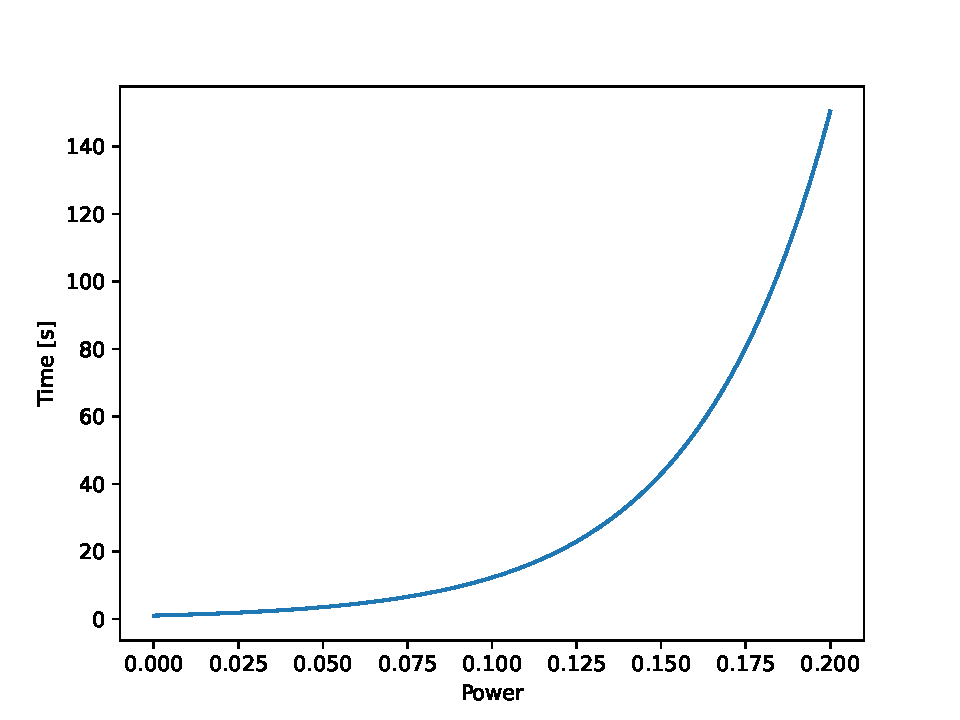
\includegraphics[width=0.5\linewidth]{1a.pdf}
                        \caption{Plot of reactivity insertion without delayed
                        neutrons}
                        \label{fig:1a}
                    \end{figure}
                \end{solution}

                \part[5] With constant delayed neutron source.
                \begin{solution}
                    With a constant delayed source, we approximate the delayed
                    neutron source as constant, that is $S_d(t) = S_{d} =
                    \beta p_{0}$. Assumuing no external source, the kinetics
                    equation becomes
                    \begin{equation}
                        \dot{p} = \frac{\rho(t) - \beta}{\Lambda}p(t) +
                        \frac{\beta p_{0}}{\Lambda}
                    \end{equation}
                    The transient following a step reactivity insertion depends
                    on the value of $\beta$. If $\beta \gg \rho$, we will have
                    an inital jump in reactivity that quickly stabilizes. As
                    $\beta > \rho$, the transient takes longer to stabilize. If
                    $\beta = \rho$, the $p(t)$ term dissappaer and we have
                    linear transient. As $\beta$ becomes less than $\rho$, the
                    transient blows up more quickly.

                    %\begin{figure}[htpb]
                    %    \centering
                    %    \subfloat[]{
                    %        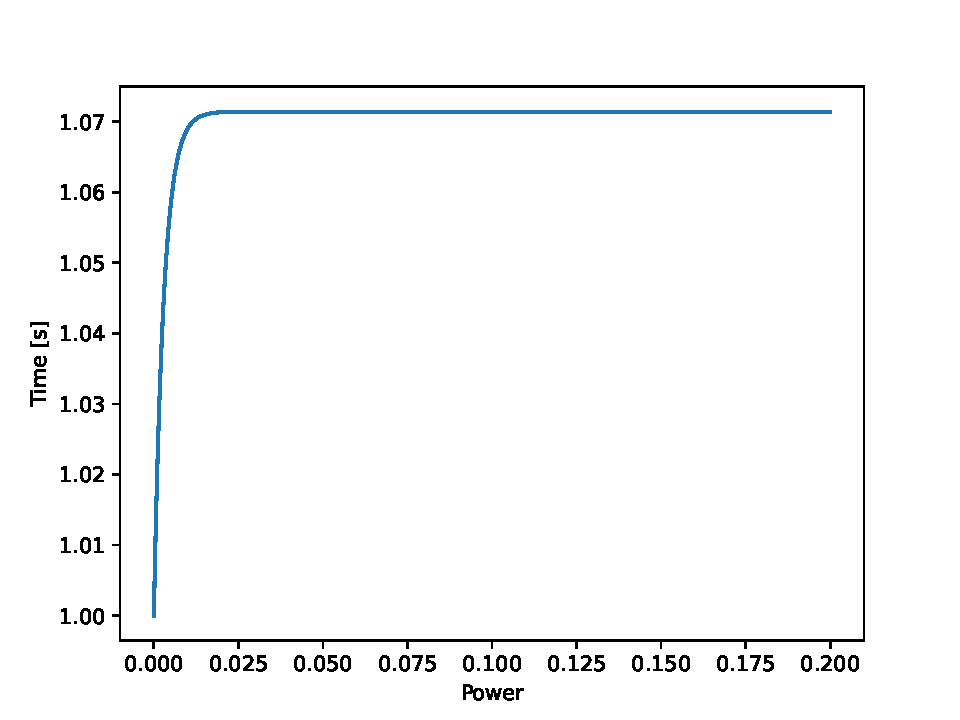
\includegraphics[width=0.5\linewidth]{1b1.pdf}
                    %        \label{fig:1b1}
                    %    }
                    %    \subfloat[]{
                    %        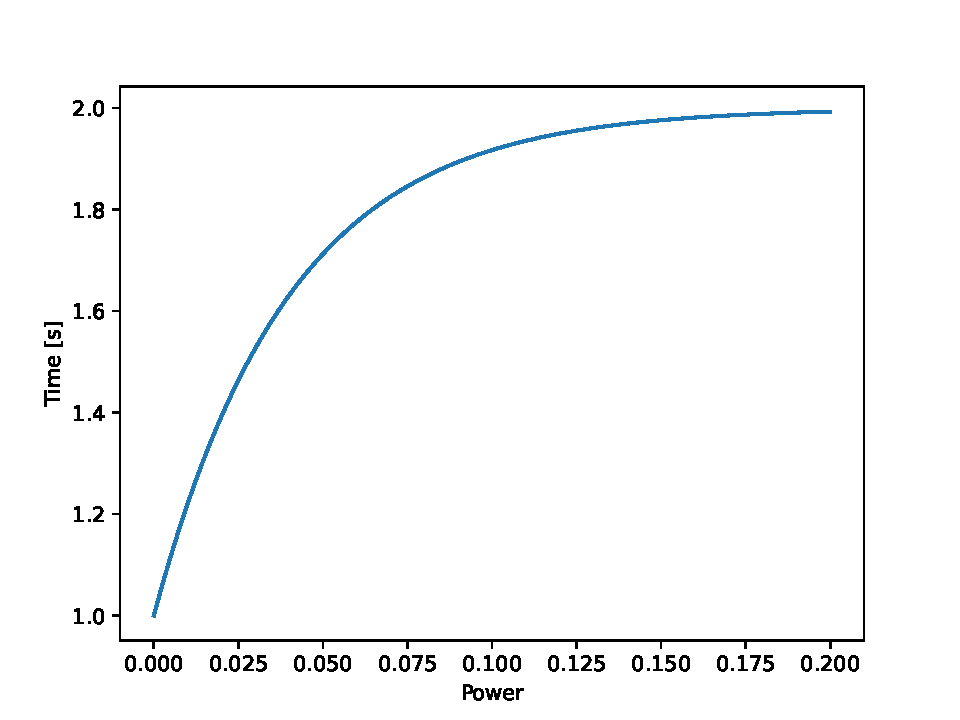
\includegraphics[width=0.5\linewidth]{1b2.pdf}
                    %        \label{fig:1b2}
                    %    }\\
                    %    \subfloat[]{
                    %        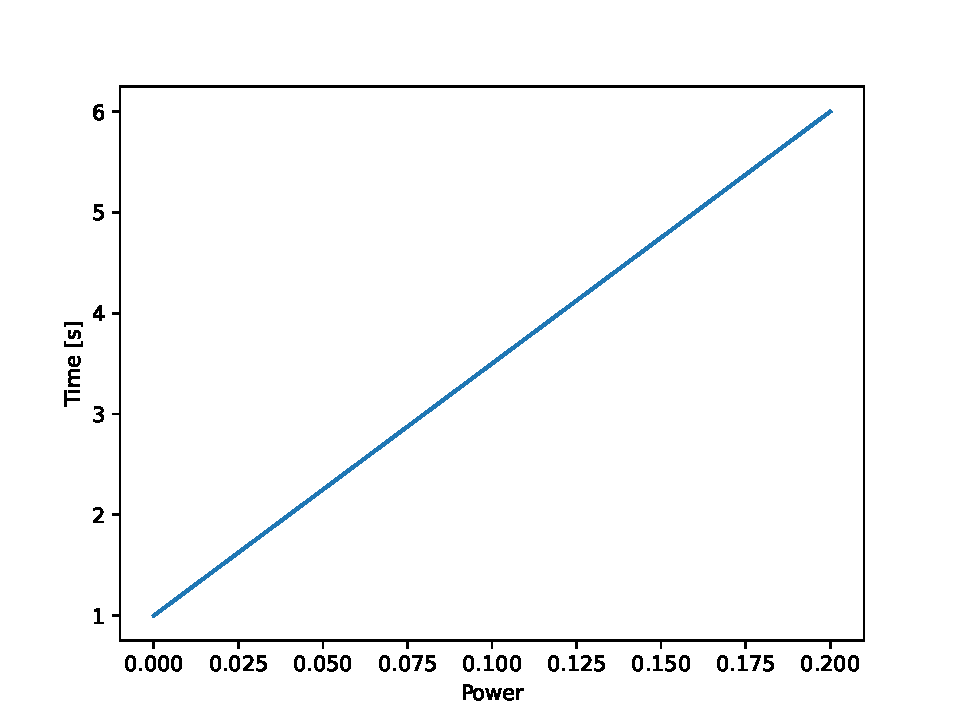
\includegraphics[width=0.5\linewidth]{1b3.pdf}
                    %        \label{fig:1b3}
                    %    }
                    %    \subfloat[]{
                    %        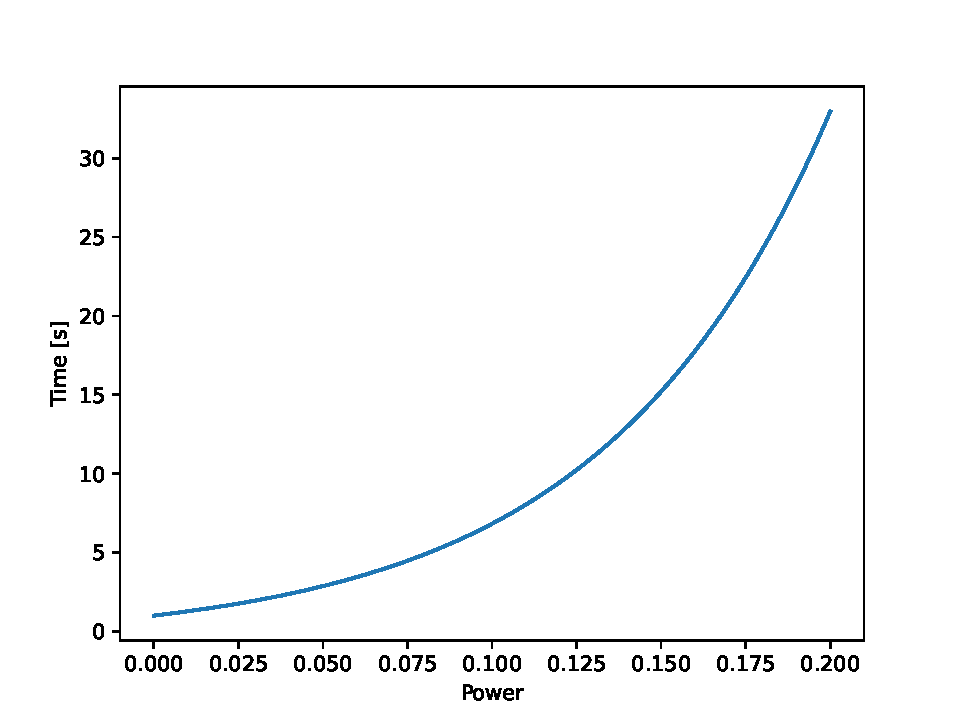
\includegraphics[width=0.5\linewidth]{1b4.pdf}
                    %        \label{fig:1b4}
                    %    }
                    %    \caption{Transients for CDS approximation, $P_0 = 1$,
                    %        $\Lambda = 2\cdot 10^{-5}$:
                    %    \subref{fig:1b1} Transient when $\beta = 750$ pcm;
                    %    \subref{fig:1b2} Transient when $\beta = 100$ pcm;
                    %    \subref{fig:1b3} Transient when $\beta = 50$ pcm;
                    %    \subref{fig:1b4} Transient when $\beta = 20$ pcm}
                    %    \label{fig:cr_eject_results}
                    %\end{figure}
                \end{solution}

                \part[5] With no approximations (no formula required).
                \begin{solution}
                        solution here
                \end{solution}

        \end{parts}

        % ---------------------------------------------
        \question (Ott Review 6.34) Estimate the time it takes to establish the 
        stable asymptotic transient for $\rho_1 < \beta$ in an initially 
        critical reactor.
                \begin{solution}
                        solution here
                \end{solution}


        % ---------------------------------------------
        \question[10] (Ott Review 6.35) Explain in terms of roots of the 
        characteristic equation:
        \begin{parts}
                \part[5] the prompt jump phenomenon
                \begin{solution}
                        solution here.
                \end{solution}
                \part[5] the delayed neutron induced transition
                \begin{solution}
                        solution here.
                \end{solution}
                \part[5] the stable period 
                \begin{solution}
                        solution here.
                \end{solution}
        \end{parts}

        
        % ---------------------------------------------
        \question[30] (Ott Problem 8.1) Find the numerical value of $p^{00}$, 
        the flux after a prompt jump for which the increase due to delayed 
        neutrons is just compensated by Doppler feedback, for an LWR from the 
        typical $\lambda$ and $\gamma/\beta$ values given in the text. Discuss 
        why $p^{00}$ may vary between reactors (e.g. the SEFOR reactor 
        discussed in the text).

        \begin{solution}
                solution here.
        \end{solution}

        % ---------------------------------------------
        \question[15] (Ott Review 8.1) Define each term, give an example of the 
        physical phenomena involved, and an example of a transient for each: 
        \begin{parts}
                \part[5] Energy coefficient.
                \part[5] Temperature coefficient. of reactvity.
                \part[5] Power coeffciient.
        \end{parts}
        \begin{solution}
                solution here.
        \end{solution}
       
       
\end{questions}



%\bibliographystyle{plain}
%\bibliography{hw01}
\end{document}
